\documentclass{article}

\usepackage{graphicx}
\usepackage{tikz}
\usepackage{tikzsymbols}
\usetikzlibrary{calc,patterns,shapes.geometric}
\pagestyle{empty}
\usepackage[margin=0pt]{geometry}
\geometry{papersize={14in,12in}}

\def\centerarc[#1](#2)(#3:#4:#5){\draw[#1] ($(#2)+({#5*cos(#3)},{#5*sin(#3)})$) arc (#3:#4:#5);}

\begin{document}
	\begin{figure}
		\centering
		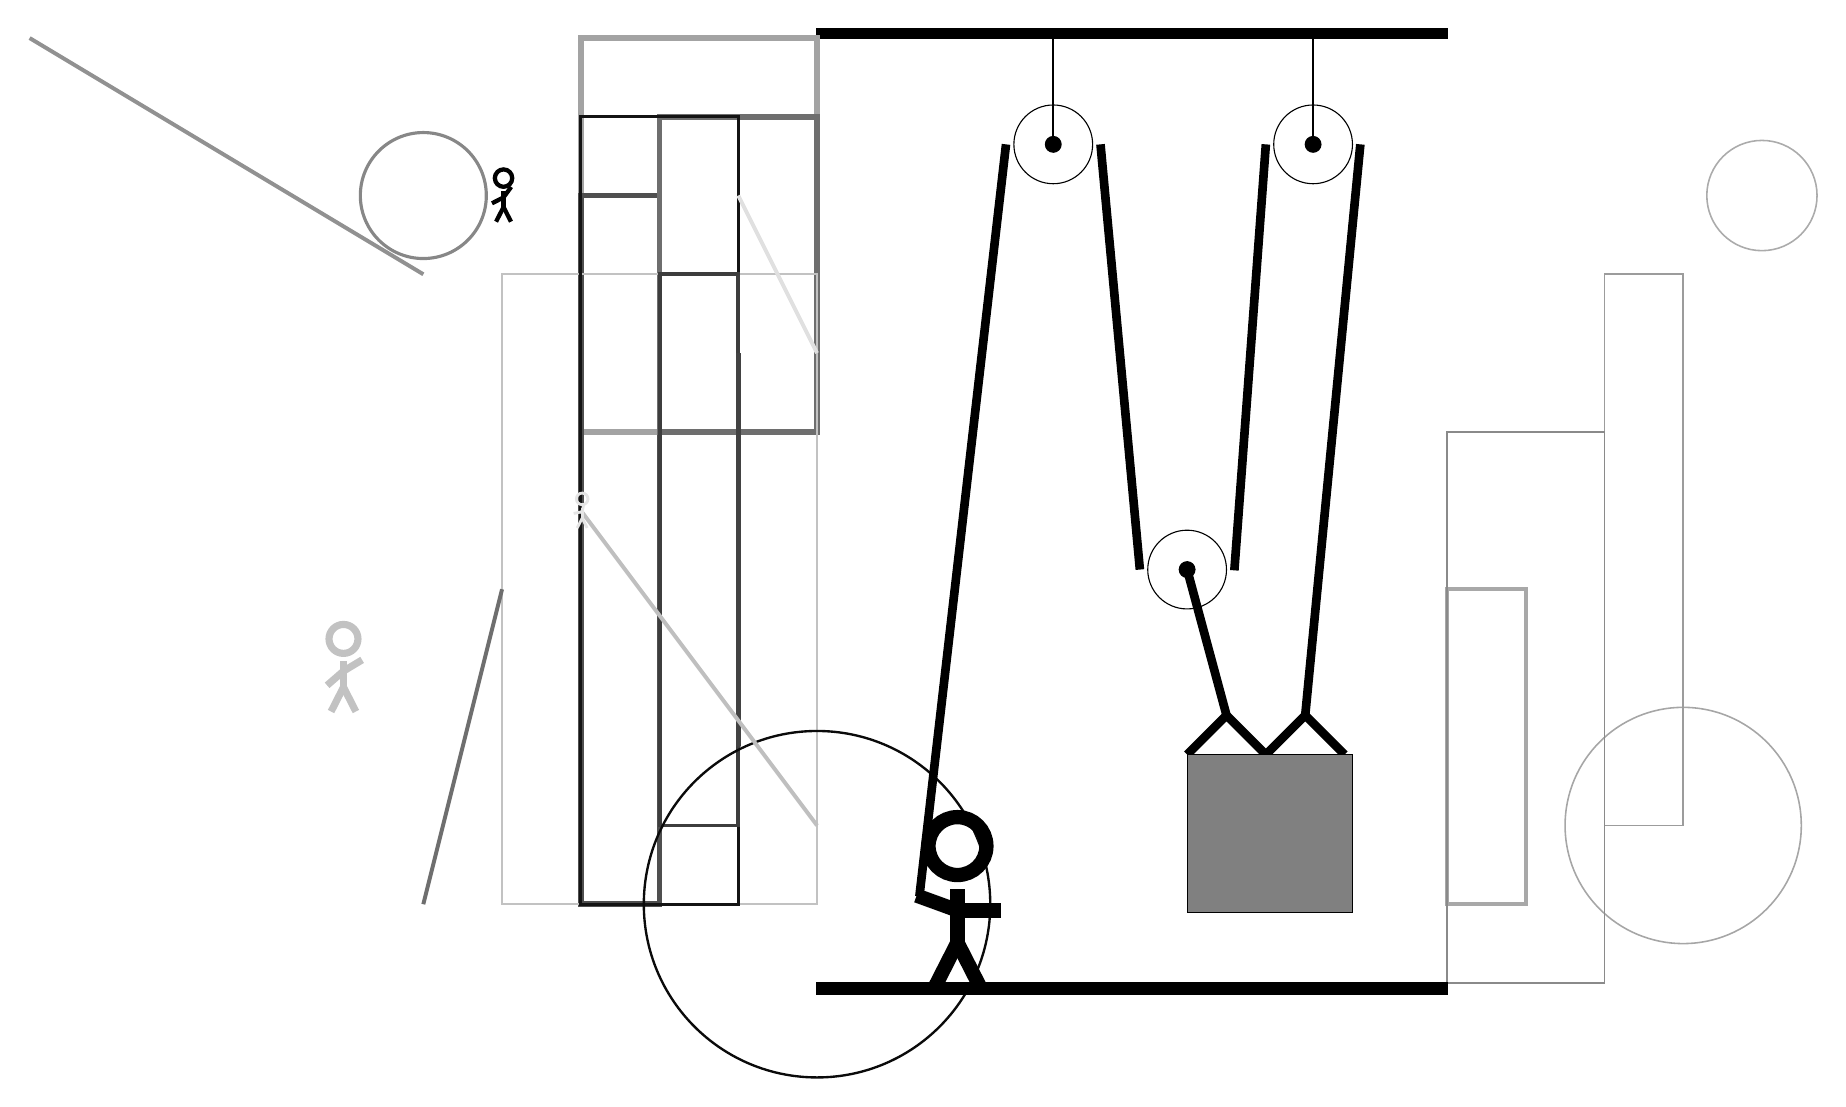
\begin{tikzpicture}
			%%%%% START %%%%%
			
			\draw[fill=black] (-2, 9) rectangle (6, 9.125);
			
			\draw (1, 7.65) circle (0.5);
			\draw[fill=black] (1, 7.65) circle (0.1);
			\draw[thick] (1, 7.65) -- (1, 9);
			
			\draw[line width=0.7mm, color=black!36] (-2, 9) rectangle (-5, 4);
			
			\draw [line width=0.2mm, color=black!35](9, -1) circle (1.5);
			\draw[line width=0.5mm, color=black!34] (6, 2) rectangle (7, -2);
			\node[line width=0.5mm, color=black!100] at (-6, 7) {\Strichmaxerl[3][27][54]};
			\draw[line width=0.7mm, color=black!69] (-4, -2) rectangle (-5, 7);
			
			\draw[line width=0.7mm, color=black!57] (-2, 8) rectangle (-4, 4);
			
			\draw[line width=0.3mm, color=black!24] (-2, 6) rectangle (-6, -2);
			
			\draw[line width=0.4mm, color=black!92] (-3, -2) rectangle (-5, 8);
			\draw [line width=0.4mm, color=black!47](-7, 7) circle (0.8);
			
			\draw[line width=0.5mm, color=black!57](-7, -2) -- (-6, 2);
			
			\node[line width=0.5mm, color=black!24] at (-8, 1) {\Strichmaxerl[5][41][31]};
			\draw[line width=0.5mm, color=black!76] (-4, 6) rectangle (-3, -1);
			\draw [line width=0.3mm, color=black!96](-2, -2) circle (2.2);
			
			\draw[line width=0.7mm, color=black!74] (-3, 0) rectangle (-3, 5);
			\draw [line width=0.2mm, color=black!33](10, 7) circle (0.7);
			\draw[line width=0.5mm, color=black!25](-5, 3) -- (-2, -1);
			
			\node[line width=0.5mm, color=black!10] at (-5, 3) {\Strichmaxerl[2][11][79]};
			\draw[line width=0.5mm, color=black!43](-7, 6) -- (-12, 9);
			\draw[line width=0.2mm, color=black!39] (8, 6) rectangle (9, -1);
			\draw[line width=0.2mm, color=black!46] (8, 4) rectangle (6, -3);
			\draw[line width=0.5mm, color=black!12](-3, 7) -- (-2, 5);
			
			
			\draw (4.3, 7.65) circle (0.5);
			\draw[fill=black] (4.3, 7.65) circle (0.1);
			\draw[thick] (4.3, 7.65) -- (4.3, 9);
			
			\draw (2.7, 2.25) circle (0.5);
			\draw[fill=black] (2.7, 2.25) circle (0.1);
			
			\draw[line width=1.1mm]  (2.7, -0.1) -- (3.2, 0.4) -- (3.7, -0.1) -- (4.2, 0.4) -- (4.7, -0.1);
			\draw[fill=black!50] (2.7, -0.1) rectangle (4.8, -2.1);
			
			\draw[line width=1.1mm](-0.7, -1.9) -- (0.4, 7.65);
			\centerarc[line width=1.1mm](1, 7.65)(0:180:0.6);
			\draw[line width=1.1mm](1.6, 7.65) -- (2.1, 2.25);
			\centerarc[line width=1.1mm](2.7, 2.25)(180:370:0.6);
			\draw[line width=1.1mm] (3.3, 2.24) -- (3.7, 7.65);
			\centerarc[line width=1.1mm](4.3, 7.65)(0:180:0.6);
			\draw[line width=1.1mm](4.2, 0.4) -- (4.9, 7.65);
			\draw[line width=1.1mm] (3.2, 0.4) -- (2.7, 2.25);
			
			\node at (-0.2, -2) {\Strichmaxerl[10][-20][0]};
			
			\draw[fill=black] (-2, -3) rectangle (6, -3.15);
			
			%%%%% END %%%%%
		\end{tikzpicture}
	\end{figure}	
\end{document}